%%%%%%%%%%%%%%%%%%%%%%%%%%%%%%%%%%%%%%%%%%%%%%%%%%%%%
%                                                   %
%     Penn State Colloquium Poster Template         %
%                                                   %
% Uses Penn State Colloquium class, with options:   %
%                                                   %
% Orientation:                                      %
%     portrait (default), landscape                 %
%                                                   %
% Paper size:                                       %
%     a4paper (default), a0paper, a1paper, a2paper, %
%     a3paper, a5paper, a6paper                     %
%%%%%%%%%%%%%%%%%%%%%%%%%%%%%%%%%%%%%%%%%%%%%%%%%%%%%
\documentclass{../psuposter}
\renewcommand{\templateimagepath}{../} 


%%%%%%%%%%%%%%%%%%%%%%%%%%%%%%%%%%%%%%%%%%%%%%%%%%%%%
%               Package Dependencies                %
%%%%%%%%%%%%%%%%%%%%%%%%%%%%%%%%%%%%%%%%%%%%%%%%%%%%%
\usepackage{natbib}
\usepackage{lipsum}                                % Dummy text
\usepackage[figwidth = 0.98\linewidth]{todonotes}  % Dummy image (and more!)
\usepackage[absolute, overlay]{textpos}            % Figure placement
\usepackage{braket}
\setlength{\TPHorizModule}{\paperwidth}
\setlength{\TPVertModule}{\paperheight}
\setcitestyle{numbers,square}


%%%%%%%%%%%%%%%%%%%%%%%%%%%%%%%%%%%%%%%%%%%%%%%%%%%%%
%                 AUTHOR AND TITLE                  %
%%%%%%%%%%%%%%%%%%%%%%%%%%%%%%%%%%%%%%%%%%%%%%%%%%%%%
\title{Scientific espionage, open exchange, and American competitiveness}
\author{Xiaoxing Xi}
\institute{Temple University}


%%%%%%%%%%%%%%%%%%%%%%%%%%%%%%%%%%%%%%%%%%%%%%%%%%%%%
%                  BEGIN DOCUMENT                   %
%%%%%%%%%%%%%%%%%%%%%%%%%%%%%%%%%%%%%%%%%%%%%%%%%%%%%
\begin{document}
\begin{frame}
\begin{columns}[t, totalwidth=\textwidth]
\begin{column}{0.45\textwidth - 1cm}


%%%%%%%%%%%%%%%%%%%%%%%%%%%%%%%%%%%%%%%%%%%%%%%%%%%%%
%                 BLOCK: BIOGRAPHY                  %
%%%%%%%%%%%%%%%%%%%%%%%%%%%%%%%%%%%%%%%%%%%%%%%%%%%%%
    \begin{block}{Speaker Biographic Summary}
    	\begin{center}
    		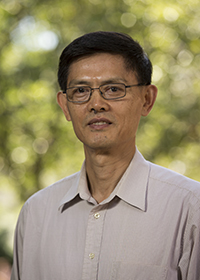
\includegraphics[width=0.55\textwidth]{images/portrait}
    	\end{center}
    	\href{https://phys.cst.temple.edu/xiaoxing-xi.html}{Dr. Xiaoxing Xi} is the Laura H. Carnell Professor of Physics at Temple University. Prior to joining Temple in 2009, he was a Professor of Physics and Materials Science and Engineering at the Penn State University. He received his PhD degree in physics from Peking University and Institute of Physics, Chinese Academy of Science, in 1987. After several years of research at the Karlsruhe Nuclear Research Center, Germany, Bell Communication Research/Rutgers University, and University of Maryland, he joined the Physics faculty at Penn State in 1995. He has received many honors, including selection as APS Fellow (2007), Chang Jiang Scholar Visiting Professor, Chinese Ministry of Education and Li Ka Shing Foundation (2006), and the NSF Career Award (1997)
    \end{block}


%%%%%%%%%%%%%%%%%%%%%%%%%%%%%%%%%%%%%%%%%%%%%%%%%%%%%
%            BLOCK: RESEARCH INTERESTS              %
%%%%%%%%%%%%%%%%%%%%%%%%%%%%%%%%%%%%%%%%%%%%%%%%%%%%%
    \begin{block}{Research Interests}
        Prof. Xi’s research focuses on the materials physics underlying the applications of oxide, boride, and transition metal dichalcogenide thin films, in particular epitaxial thin films and heterostructures at the nanoscale. Using various deposition techniques including Laser Molecular Beam Epitaxy and Hybrid Physical-Chemical Vapor Deposition, his group is currently working on the atomic layer-by-layer growth of artificial oxide heterostructures, magnesium diboride thin films for electronic and radio frequency cavity applications, iron pnictide superconductor thin films for phase sensitive measurements, and thin films of 2D layered materials transition metal dichalcogenides. 
        %He has published over 300 papers in refereed journals, book chapters, and conference proceedings, and holds three patents in the area of thin films of high-Tc superconductors and magnesium diboride.
        \begin{center}
	    	
\includegraphics[width=0.15\textwidth]{images/research}    
	    	
	    	\textit{Caption.} 
    	\end{center}
    	
    \end{block}
\end{column}
\begin{column}{0.55\textwidth - 1cm}


%%%%%%%%%%%%%%%%%%%%%%%%%%%%%%%%%%%%%%%%%%%%%%%%%%%%%
%                 BLOCK: ABSTRACT                   %
%%%%%%%%%%%%%%%%%%%%%%%%%%%%%%%%%%%%%%%%%%%%%%%%%%%%%
    \begin{block}{Talk Abstract}
    	Amid rapidly escalating tension between the United States and China, professors, scientists, and students of Chinese ethnic origin as well as those engaging in academic collaborations with China are under heightened scrutiny by the federal government. Law enforcement officials consider collaborating with Chinese colleagues “by definition conveying sensitive information to the Chinese.” In 2015, I became a casualty of this campaign despite being innocent. This experience gave me insights into the challenges Chinese scientists face and the immediate threat to the open environment in fundamental research. In this talk, I will urge the audience to rally around the JASON Report commissioned and endorsed by the NSF and speak up to defend Chinese colleagues against injustice, safeguard open fundamental research on university campuses, and protect American leadership in science and technology.
    \end{block}


%%%%%%%%%%%%%%%%%%%%%%%%%%%%%%%%%%%%%%%%%%%%%%%%%%%%%
%                BLOCK: BACKGROUND                  %
%%%%%%%%%%%%%%%%%%%%%%%%%%%%%%%%%%%%%%%%%%%%%%%%%%%%%
    \begin{block}{Brief Background}
    In May 2015, the United States Department of Justice (DOJ) wrongfully, accused Prof. Xi of sending restricted American technology to China: specifically, the design of a pocket heater used in superconductor research. Prof. Xi was arrested and faced charges carrying a maximum penalty of 80 years in prison and a \$1 million fine. He was put on administrative leave by Temple University and resigned as chairman of the physics department. In the following years, however, the DOJ dropped all charges against him after leading scientists, including a co-inventor of the pocket heater, provided affidavits that the schematics that Xi shared with Chinese scientists were not for a pocket heater or other restricted technology. Ever since then, he has advocated for other Chinese-American researchers targeted by the government.
    	
    	%\cite{longLocalAxonalConduction2020} 
        \begin{center}
		   	
\includegraphics[width=0.45\textwidth]{images/background}    		
    	\end{center}
		Following his experience being falsely accused as a spy by the FBI, Xiaoxing Xi will speak to us on defending Chinese colleagues against injustice, safeguarding open fundamental research on university campuses, and protecting American leadership in science and technology.  
		%\cite{longMorphologicalCharacterizationHVC2018} 
    \end{block}


%%%%%%%%%%%%%%%%%%%%%%%%%%%%%%%%%%%%%%%%%%%%%%%%%%%%%
%                 BLOCK: REFERENCES                 %
%%%%%%%%%%%%%%%%%%%%%%%%%%%%%%%%%%%%%%%%%%%%%%%%%%%%%
    \begin{block}{References}
        \bibliographystyle{aipnum4-1}
%        \bibliographystyle{iopart-num}
		\bibliography{references}
    \end{block}

\end{column}
\end{columns}


%%%%%%%%%%%%%%%%%%%%%%%%%%%%%%%%%%%%%%%%%%%%%%%%%%%%%
%                    FOOTER TEXT                    %
%%%%%%%%%%%%%%%%%%%%%%%%%%%%%%%%%%%%%%%%%%%%%%%%%%%%%
\begin{textblock}{0.5}(0.18, 0.94)
    \color{white}
    \sffamily
    \textbf{Eberly College of Science}
    \\
    Department of Physics
\end{textblock}


%%%%%%%%%%%%%%%%%%%%%%%%%%%%%%%%%%%%%%%%%%%%%%%%%%%%%
%                   END TEMPLATE                    %
%%%%%%%%%%%%%%%%%%%%%%%%%%%%%%%%%%%%%%%%%%%%%%%%%%%%%
\end{frame}
\end{document}
